% Artifact mockup only. Not input by main.tex.
% Table 17 remains in the manuscript PDF.
\documentclass[11pt]{article}
\usepackage[margin=1in]{geometry}
\usepackage[utf8]{inputenc}
\usepackage[T1]{fontenc}
\usepackage{mathptmx}
\usepackage{graphicx}
\usepackage{microtype}
\usepackage[font=small,labelfont=bf,labelsep=period]{caption}

\begin{document}
\pagestyle{empty}

\noindent\textit{Mockup page (not in the manuscript PDF). Table~17 remains in the paper.}

\vspace{1.2em}

\begin{figure}[h]
\centering
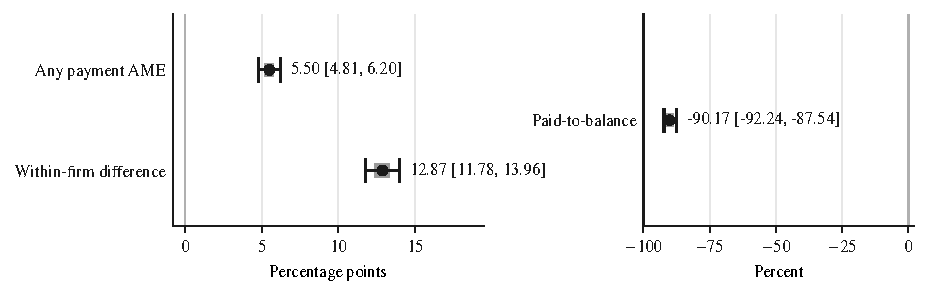
\includegraphics[width=\textwidth]{fig_origin_contrasts_v3.pdf}
\caption{Assessed origin relative to declared origin.
The left panel reports the average marginal effect on any payment and the within-firm difference in the probability of any payment, in percentage points.
The right panel reports the percentage difference in expected payments per real of stock.
Declared origin is the reference.
The marker is the point estimate.
The thin line with caps is the cluster 95~percent interval.
The thicker gray segment is the HC3 95~percent interval.
Each panel includes zero on the horizontal axis.
The quantile regression of log stock is a separate equation.}
\end{figure}

\end{document}
